\documentclass[10pt]{article}
\usepackage[utf8]{inputenc}
\usepackage[T1]{fontenc}
\usepackage{graphicx}
\usepackage[export]{adjustbox}
\graphicspath{ {./images/} }
\usepackage{amsmath}
\usepackage{amsfonts}
\usepackage{amssymb}
\usepackage[version=4]{mhchem}
\usepackage{stmaryrd}

\title{Newton's Method in Machine Learning }

\author{Ibrahim Ahmad, Cipriano Dorbessan, Christopher Gossmann}
\date{April 2025}


\begin{document}
\maketitle
\section{Introduction}
In this project, we explored and tested the practical effectiveness of Newton's Method as an optimization technique within the machine learning context. We were interested in investigating whether this second-order method could be effectively adapted and optimized to train neural networks on a simple supervised learning problem: digit classification using the digits dataset.

To do this, we developed a feedforward neural network and trained it on the digits dataset provided by scikit-learn. What we focused our project on is the implementation of our own Newton's Method optimizer, including the computation of gradients and Hessians, and solving the resulting linear systems at each iteration. For this we had to learn the mathematical foundations of Newton's Method and numerical differentiation, matrix manipulation, and computational efficiency.

Once we had a working implementation, we compared the performance of our Newton-based optimizer against two widely used optimization algorithms in machine learning: Stochastic Gradient Descent (SGD)\cite{contributors-2020-stochastic} and ADAM \cite{kingma2017adammethodstochasticoptimization}. By training and testing the model with the different optimizers, we observed that our optimizer was able to reduce training error over time and showed the convergence properties we were looking for. However, despite these results we achieved, our optimizer did not reach the level of performance achieved by ADAM or SGD in terms of accuracy, and also our optimizer took a lot more time to train when compared to these others.

This outcome shows that using Newton's Method for machine learning is possible, but might not be ideal. While it also uses the second-order derivative to converge, it is made worse because of the computational complexity of calculating the Hessian matrix-especially in higher dimensions. However, this project can serve as insight on the potential challenges of incorporating second-order optimization techniques into neural network training.
\newpage
\subsection{Background of Newton's Method and complexity in Machine Learning}
Previously we knew that Newton’s method optimization requires the following data: an initial guess for the minimum of the function, a tolerance level for convergence, and a maximum number of iterations. Here, the initial guess is randomly generated, but the further the guess is from the actual minimum, the longer it may take for Newton’s method to find the minimum.

Newton’s method converges to a solution at least quadratically (this holds only for the neighborhood of the root)\cite{geeksforgeeks-2024-newtons}, in that each iteration the number of accurate digits approximately doubles. Nevertheless, this can be affected by a variety of factors. As mentioned in the previous paragraph, if the initial guess is very close to the solution, the number of iterations may be very few, but if it’s very far, it may not only cause slow convergence, but even divergence and never find the minimum of the function. Additionally, Newton’s method, because it’s based on differentiation, relies on the function to have continuous first and second derivatives, so it is very inefficient or cannot be used at all if the function has discontinuities or singularities. Lastly, Newton’s method ends when the change in the predicted solution is small enough or when the value of the prediction is very close to 0. Newton’s method’s performance may also vary depending on the shape of the function. Functions with a relatively linear first derivative may have faster convergence in the input space, as the tangent line approximation of the first derivative by the second derivative is more accurate.

Because Newton’s method has a quadratic convergence rate, it is considered to be a good choice based on the number of iterations needed to find the solution, however it can still have greater complexity than other optimization algorithms. This is mainly because each iteration requires calculating both the gradient (first derivative) and the Hessian (second derivative), so it can be very computationally expensive when used with a lot of variables. Also, the manipulation and storage of the Hessian matrix is very memory-expensive, especially for high dimensions. With n variables, calculating the gradient is $O(n)$ and calculating the Hessian is $O(n^2)$. Lastly, solving the linear systems with any method is usually $O(n^3)$ when it’s dense. The number of iterations can vary greatly, as it depends on the tolerance level, curvature of the function, and the initial guess.

\section{Proofs}
There are a few nontrivial statements that are crucial for understanding Numerical Optimization and training Neural Networks.
\subsection{Proof Of Taylor's Theorem}
Taylor's Theorem is cruicial for doing numerical optimization \cite{recht-wright}. It allows us to provide an approximation of a function in the open neighbourhood of a point.

We must prove Taylor's theorem for the high dimensional case. We shall do so directly.
Let $f : \mathbb{R}^n \mapsto \mathbb{R}$. We shall observe some properties of $f$ in the region of $A$, where $A$ is an open subset of $\mathbb{R}^n$. We shall make the following assumptions: $f$ is continuous on $A$, $f$ is differentiable on $A$. (Note: We do not contain the boundary points as this allows us to handle asymptotics more neatly). 
Let us define the derivative of $f$ in the direction of $\alpha$ by writing \begin{equation}\vec{\alpha} \cdot \vec{\nabla} f(\vec{x}) = \lim_{t \to 0}\frac{f(\vec{x} + \vec{\alpha}t) - f(\vec{x})}{t}\end{equation}, under the assumption that $\vec{x} + t \vec{\alpha} \in A$. This allows us to find the derivative in any direction from the location of $x$. Let us define $\Phi(t) = f(\vec{x} + \vec{\alpha} t)$. Because $\Phi : \mathbb{R} \mapsto \mathbb{R}$
we can use the one dimensional form of Taylor's theorem \cite{wikipediacontributors-2019-taylor}on $\Phi$. This lets us write the equivalency 
\begin{equation}\Phi(t) = \Phi(0) + \Phi'(0)t + \Phi''(0)\frac{t^2}{2} + \dots\end{equation}
By substituting the definition of $\Phi(t)$ into both sides, we can write 
\begin{equation} f(\vec{x} + t \cdot \vec{\alpha}) = \Phi(0) + \Phi'(0)t + \Phi''(0)\frac{t^2}{2} + \dots\end{equation}
We also know that 
\begin{equation}\Phi(t)' = \lim_{t \to 0}\frac{f(\vec{x} + \vec{\alpha}t) - f(\vec{x})}{t} = \vec{\alpha} \cdot \vec{\nabla}f(\vec{x})\end{equation}
By the definition of $\Phi$, and $\vec{\alpha} \cdot \vec{\nabla}$.
By substituting into both sides, we get the following. For convenience, we shorten $\vec{\alpha}\cdot\vec{\nabla}$ to $\vec{\nabla}$.
\begin{equation} f(\vec{x} + t \cdot \vec{\alpha}) = f(\vec{x}) + [\vec{\nabla}f(\vec{x})]^T\vec{\alpha} t + \frac{1}{2}\vec{\alpha}^T[\vec{\nabla}^2f(\vec{x})]\vec{\alpha} \cdot t^2 + \dots\end{equation}
We shall only use first and second order methods, so we have not shown the third order term of the Taylor Series, which requires rank 3 tensor multiplications.
Thus we have proved Taylor's Theorem for functions $f : \mathbb{R}^n \mapsto \mathbb{R}$, under an open subset of $\mathbb{R}^n$.


\subsection{Convergence Of Gradient Descent}
While we do not use Gradient Descent to train any of the models, understanding Gradient Descent and it's properties is crucial to understanding Adam, Stochastic Gradient Descent, and Newton's Method. For further reading regarding these algorithms we reccomend \cite{recht-wright}  and \cite{wikipediacontributors-2019-newtons}.

Because the Neural Network is not L-Smooth\cite{lipschitz}, or Convex, we must show the convergence of Gradient Descent under minimal assumptions. Let $x_k$ be the value of the descent's algorithm's value at the $k$'th iteration. We shall use the following update rule $x_{k+1} = x_k - \eta_k\vec{\nabla}f(x_k)$.


By the mean value theorem \cite{wikipediacontributors-2019-mean}, we know that $f(\vec{x_{k+1}}) = f(\vec{x_k}) - \eta \|\vec{\nabla}f(x_k)\|^2 + o(\eta\|\vec{\nabla}f(\vec{x_k}\|^2)$. The proof of the $o$ term is complex and not useful for what we intend to do, but is discussed in . It can be imagined as an upper bound of the remainder of the Taylor approximation $f(x_{k+1})$ after the first term. If $\eta_k$ is sufficently small, we can write $f(x_{k+1}) \leq f(x_k) - \eta_k \|\vec{\nabla}f(x_k)\|^2$. We must make the assumption that $\eta_k$ is sufficently small, as without that assumption we may overshoot the point we intend on converging to. We note, that under these assumptions $f(x_{k+1}) < f(x_k)$ if $\eta_k \|\vec{\nabla}f(x_k)\|^2$ is nonzero, and $f(x_{k+1}) = f(x_k)$ if $\eta_k \|\vec{\nabla}f(x_k)\|^2$ is zero. Thus we have shown that the function values are decreasing, and the algorithm converges at a minima or saddle point if $f$ is lower bounded.

We note that $\lim_{k \to \infty} \|\vec{\nabla}\| = 0$, as that is the state the algorithm must converge to to be considered to have converged.
We also know that $\eta_k > 0$, as if $\eta_k = 0$, then the algorithm would not converge.

\subsection{Convergence Of Other Descent Algorithms}

We shall now study the convergence of algorithms of the following form $x_{k+1} = x_k - S_k\vec{\nabla}f(x_k)$. The constraints we place are that $S_k\vec{\nabla}f(x_k)$ is sufficiently small as to not overshoot the extrema, and that $S_k$ is a positive definite matrix. For example, Newton's method chooses $S_k = \vec{\nabla}^{-2}f(x_k)$.

Algorithms that follow this form are guarunteed to converge to a minima such that $\vec{\nabla}f(x_k) = 0$. Recall the following property of positive definite matrices, for some arbitrary vector $\vec{v}$, $\vec{v}^TS\vec{v} > 0$. In other words, when multiplying the matrix $S$ by some vector, that vector is rotated by less than $90^{\circ}$. Thus we know that $(S_k\vec{\nabla}f(x_k)) \cdot \vec{\nabla}f(x_k) > 0$. Let us now project $S_k\vec{\nabla}f(x_k)$ onto $\vec{\nabla}f(x_k)$, yielding $d_k$. Because $S_k$ is semi definite, we know that $d_k$ is nonzero and $d_k \cdot ,\vec{\nabla}f(x_k)$ or in other words, $S_k$ transforms the gradient vector such that it no longer faces the direction of steepest descent, but it still faces a direction of descent. Because the projection in the descent direction is a nonzero positive scaled version of the gradient, the descent can be considered to be similar to that of gradient descent with a different stepsize.

\section{Network model}
We used Tensorflow with Keras to build our network model. The dataset we used was "Pen-Based Recognition of Handwritten Digits" which consists of 8x8 images of handwritten digits. Our network consists of an input layer of 64 neurons (one for each pixel), a hidden layer of 32 neurons with ReLU as their activation function, and an output layer of 10 neurons (one for each digit) with softmax as the activation. For the ADAM and SGD optimizers, we used Keras' built-in optimizers. We wrote the Newton's Method optimizer ourselves using Keras' automatic differentiation (through the use of Gradient Tapes and the built-in Jacobian method). The Adam and SGD models were trained using Tensorflow's fit method, and the Newton's method model was trained using our own train function, as there was no pre-existing function to do this. When analyzing the results, it is important to take into account that the networks using ADAM and SGD will have a slight advantage over the network using our custom Newton's Method optimizer, as the code for these two optimizers was written and optimized by Tensorflow developers over many years.

\section{Results and conclusions}
We trained and evaluated the model's performance over the course of 50 training epochs, comparing our Newton's Method optimizer with ADAM and Stochastic Gradient Descent (SGD). The results, shown in the training loss and accuracy plots, reveal several important insights into the strengths and limitations of each approach.\\
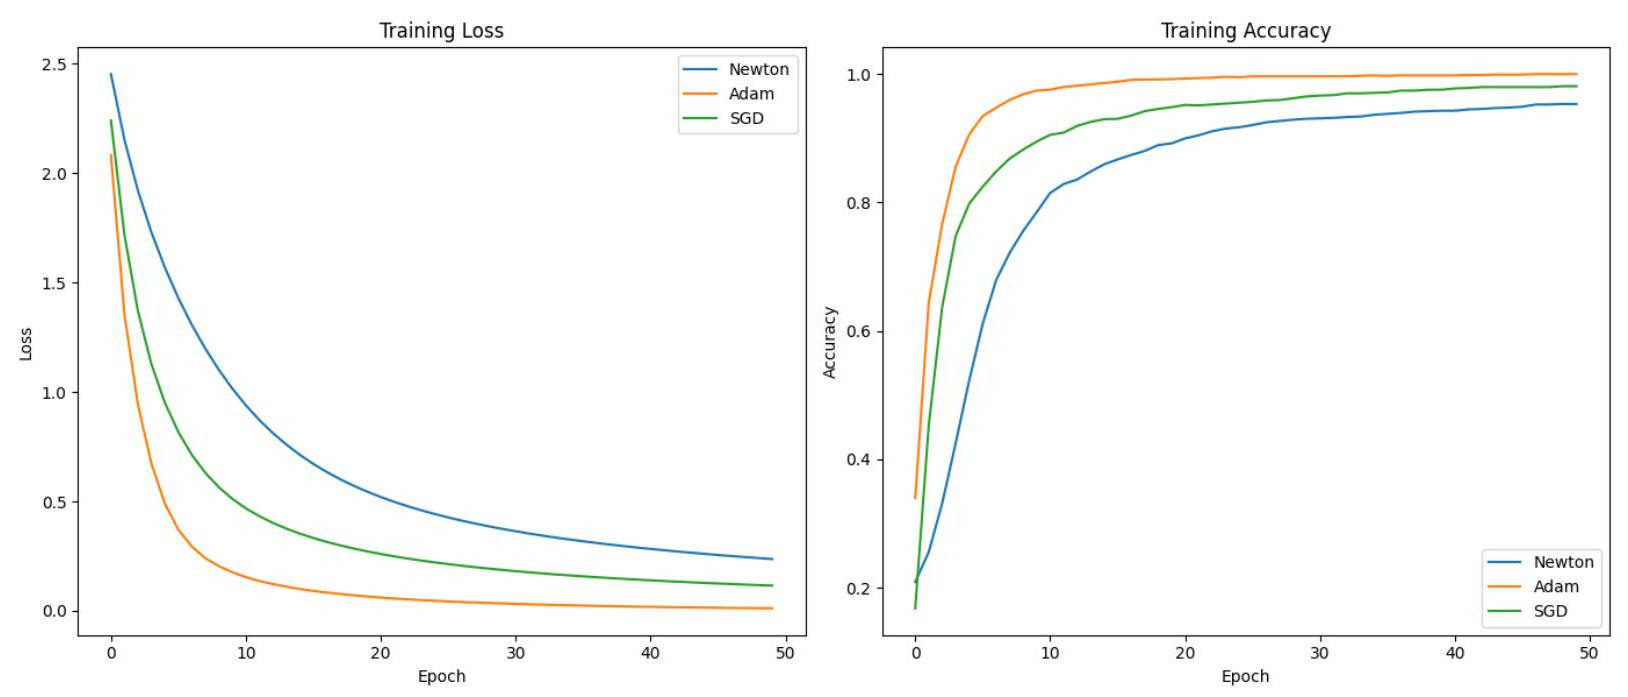
\includegraphics[max width=\textwidth, center]{2025_04_08_c5129b05008e68f8b3cdg-2}

From the training loss graph, it can be seen that ADAM achieved the fastest and most stable convergence, reducing the loss to near zero within the first 20 epochs. SGD also performed well, it still converged slower than ADAM but still significantly reduced the loss over the epochs. Newton's Method, while improving the loss steadily, underperformed when compared to both ADAM and SGD, as it showed a slower rate of convergence.

Similarly, the training accuracy graph highlights that ADAM quickly pushed the model to over $95 \%$ accuracy, with SGD really close to it. Newton's Method displayed a more gradual improvement in accuracy, reaching around $93 \%$ by the end of training. While this is a very good result, it always performed worse than the other two optimizers.

These results suggest that while Newton's Method has theoretical advantages, such as quadratic convergence near the optimal values, its practical application in training neural networks is limited by the computational cost of its operations and because the initial conditions affect it greatly. The cost of calculating the Hessian matrix at each step likely contributed to its slower performance.

Despite this, our implementation demonstrated that Newton's Method is capable of reducing error and improving accuracy just by calculating the gradient and the hessian, and without using any adaptive strategies like ADAM.

In conclusion, our project shows that Newton's Method works as an optimization algorithm in machine learning but may not be ideal, especially when compared with modern first-order optimizers for large-scale and real-time training tasks, as these take much less time than our custom Newton's method optimizer.

\section{Extensions and Applications}
Once again, the performance of the Newton's Method optimizer was heavily impacted by the fact that we wrote the optimizer ourselves, rather than using a pre-written optimizer. A direct extension on our project would be to optimize our optimizer. One such way to do this is to code it in a faster language like $\mathrm{C} / \mathrm{C}++$ and to improve on the calculation of the hessian.

Other extensions include using Newton's Method in other machine learning contexts, such as non-classification neural networks such as regression, or even in unsupervised or reinforcement learning. Another possible extension is the use of other optimization algorithms to train networks, such as derivative-free algorithms. Newton's Method is also used for Interior-Point solvers\cite{ipopt} like Sleipnir \cite{sleipnir}. 

\bibliographystyle{IEEEtran}
\bibliography{main}

\end{document}
